\section{Results}
\begin{figure}
	\centering
	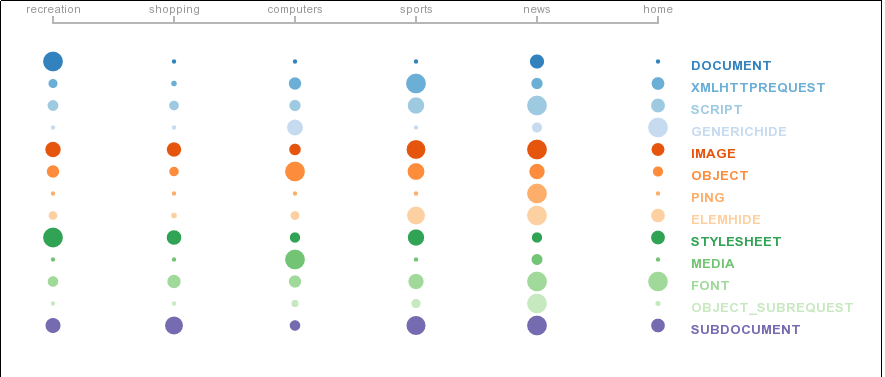
\epsfig{file=figures/abp_filters.png, width=0.50\textwidth}
	\vspace*{-0.5cm}
	\caption{\textbf{Filter Types in Adblock Plus}}
	\label{fig:abp-filters}
	\vspace*{-0.5cm}
\end{figure}
\begin{figure}
	\centering
	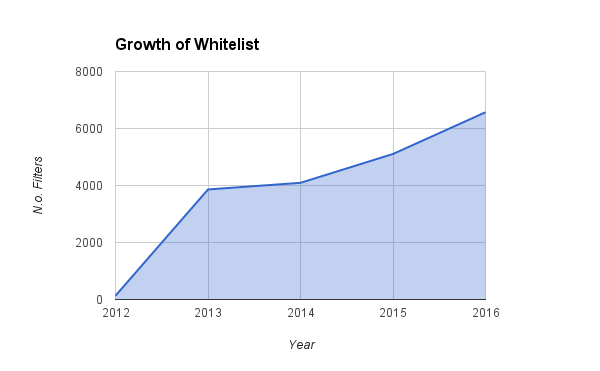
\epsfig{file=figures/growth.png, width=0.50\textwidth}
	\vspace*{-0.5cm}
	\caption{\textbf{Growth of Whitelist.}}
	\label{fig:growth}
	\vspace*{-0.5cm}
\end{figure}
\begin{figure}
Figure~\ref{fig:abp-filters} indicates the different types of filters  present in adblock.
The horizontal axis lists the domains associated with the webpages and the vertical axis lists the type of filter fired. The size of the circle corresponds to  the proportion of elements in that domain that are of a particular element type as indicated in the corresponding vertical axis. Looking at  particular domain from top to bottom shows the composition of various elements in the web pages belonging to that domain. In most of the cases  SCRIPT,IMAGE and SUBDOCUMENT can be seen as the dominating elements. These are the elements which the Adblock plus browser addon counts as an advertisement as a part of its statistics gathering.

Figure~\ref{fig:growth}, indicates the growth of whitelist since 2012. The aacceptable ads program had initially 132 filters in it. Over the years the whitelist has grown enormously in  size.  Over 3600 filters were added  between 2012 to 2013 and the list has been growing. As of March 2016, the total number of  filters in the whitelist is 6570.
Unsurprisingly, one can see an increasing trend in the number of ads allowed by adblock plus.
Figure~\ref{fig:ads-allowed}, shows the trend in the ads allowed over the years.

	\centering
	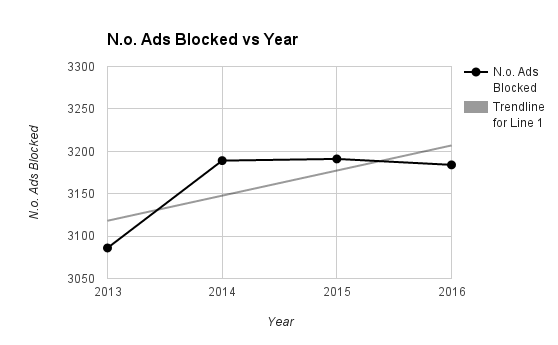
\epsfig{file=figures/alexa_ads.png, width=0.50\textwidth}
	\vspace*{-0.5cm}
	\caption{\textbf{Number of Ads allowed in the Alexa top 200.}}
	\label{fig:ads-allowed}
	\vspace*{-0.5cm}
\end{figure}

~\ref{fig:block-allow} shows the difference between the number of  elements  blocked  versus the number of elements allowed for three different  combuinations of the filters.
It can be seen that the list with only the element hiding filter does poorly in blocking the  elements as it does not have the capabilities of blocking URLS.
As expected the easylist+whitelist combination allows more ads there by allowing more elements.
\begin{figure}
	\centering
	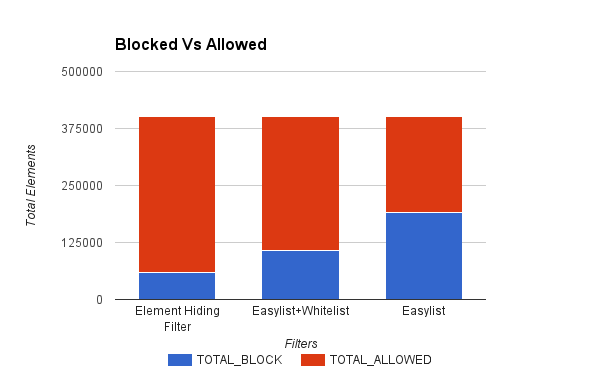
\epsfig{file=figures/exp_comparison.png, width=0.50\textwidth}
	\vspace*{-0.5cm}
	\caption{\textbf{Blocked vs Allowed for filter combinations}}
	\label{fig:block-allow}
	\vspace*{-0.5cm}
\end{figure}